\section{PKCS\#7 Padding and Padding Validation}

AES operates on 16-byte blocks, but real messages are rarely an exact multiple of 16 bytes. Padding solves this mismatch by extending the message to the next block boundary. In PKCS\#7 padding, if $k$ bytes are needed, then the sender appends $k$ copies of the byte value $k$. The receiver decrypts the final block, reads the last byte, and checks whether the last $k$ bytes are all equal to $k$.

\begin{figure}[H]
    \centering
    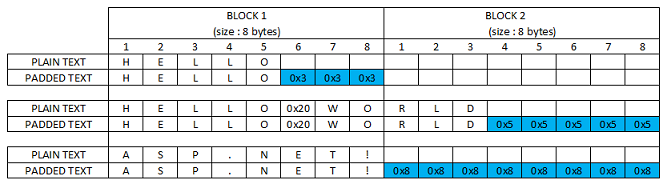
\includegraphics[width=0.8\textwidth]{images/pkcs7_padding.png}
    \caption{Example of PKCS\#7 padding patterns for different message lengths.}
    \caption*{\footnotesize Source: Bilgehanturan, Wikimedia Commons, \emph{Padding en.png} (CC BY-SA 4.0).}
    \label{fig:pkcs7}
\end{figure}

The padding rule itself is straightforward. The security issue appears during decryption. If the last byte claims that the padding length is 4, then the receiver must verify that the last four bytes are all equal to \texttt{04}. If they are not, the receiver rejects the ciphertext. From a software-engineering point of view, this validation seems harmless. From a cryptographic point of view, it can be dangerous because the rejection leaks information about the decrypted plaintext.

The key observation is that the attacker does not need a detailed error message. A single-bit answer is enough:

\begin{center}
\textit{``Did the modified ciphertext produce valid padding: yes or no?''}
\end{center}

That bit may leak through an explicit error page, a protocol alert, a timing difference, a dropped connection, or a change in application behavior. Once the attacker can distinguish valid padding from invalid padding, the receiver has effectively become a padding oracle.

The padding check is therefore not the root problem by itself. The real problem is the combination of three properties:

\begin{itemize}
    \item CBC malleability,
    \item unauthenticated decryption, and
    \item observable validation behavior.
\end{itemize}

When these three properties coexist, the attacker can learn plaintext without ever recovering the secret key.
